\section{Lezione 9}
\subsection{Approfondimento: formula di Taylor con resto di Lagrange}
\begin{theorem}
    \label{th:9n.1}
    Sia $f\colon[a,b]\to\mathbb{R}$ una funzione tale che la derivata $n$-esima $f^{(n)}$ sia continua su $[a,b]$ e tale che $f^{(n+1)}\colon(a,b)\to \mathbb{R}$ sia ben definita. Siano $\alpha, \beta\in[a,b]$ con $\alpha<\beta$; definiamo come in \eqref{eq:6.7} il polinomio di Taylor $P(x)$ di grado $n$ e centro $\alpha$,
    \[
    P(x) = \sum_{k=0}^n \frac{f^{(k)}(\alpha)}{k!}(x-\alpha)^k
    \]
    Allora esiste $\xi\in(\alpha, \beta)$ tale che 
    \[
    f(\beta) = P(\beta)+\frac{f^{(n+1)(\xi)}}{(n+1)!}(\beta-\alpha)^{n+1}
    \]
\end{theorem}
\begin{proof}
    Innanzitutto, consideriamo la seguente equazione in $k\in\mathbb{R}$:
    \begin{equation}
        \label{eq:9n.1}
        f(\beta)=P(\beta)+k(\beta-\alpha)^{n+1}
    \end{equation}
    Notiamo che dato che $\beta\ne \alpha$ questa ammette una soluzione $\overline{k}$, ossia esiste $\overline{k}\in\mathbb{R}$ tale che
    \begin{equation}
        \label{eq:9n.2}
        f(\beta)-P(\beta)-\overline{k}(\beta-\alpha)^{n+1}=0
    \end{equation}
    Per dimostrare il teorema è quindi sufficiente dimostrare che
    \[
    \overline{k} = \frac{f^{(n+1)}(\xi)}{(n+1)!}
    \]
    per qualche $\xi\in(\alpha,\beta)$. A questo scopo, definiamo la funzione $g\colon [a,b]\to \mathbb{R}$,
    \[
    g(t) = f(t)-P(t)-\overline{k}(t-\alpha)^{n+1}
    \]
    Dato che $f\in \mathscr{C}^n([a,b])$, allora $g\in\mathscr{C}^{n}([a,b])$ (i.e. $g^{(n)}$ è continua su $[a,b]$, e quindi esistono e sono continue le derivate precedenti), e inoltre $g^{(n+1)}\colon(a,b)\to\mathbb{R}$ è ben definita. Notiamo che, poiché $P(t)$ è un polinomio di grado $n$, $\frac{d^{n+1}}{dt^{n+1}}P(t)=0$; pertanto
    \[
    g^{(n+1)}(t) = f^{(n+1)}(t)-\overline{k}(n+1)!
    \]
    Inoltre, vale che $g^{(i)}(\alpha)=0$ per ogni $i\in\{0, \dots, n\}$: infatti,
    \[
    g^{(i)}(\alpha)=f^{(i)}(\alpha)-\frac{d^i}{dt^i}P(t)\bigg|_{t=\alpha}-\overline{k}\frac{(n+1)!}{(n+1-k)!}(t-\alpha)^{n+1-k}\bigg|_{t=\alpha}
    \]
    Notiamo che
    \[
    \frac{d^i}{dt^i}P(t)\bigg|_{t=\alpha} = \sum_{k=0}^n \frac{f^{(k)}(\alpha)}{k!}\frac{d^i}{dt^i}(t-\alpha)^{k}\bigg|_{t=\alpha} 
    \]
    ove
    \[
    \frac{d^i}{dt^i}(t-\alpha)^k = \begin{dcases}
        0\, & k<i\\
        i!\, &k=i\\
        \frac{k!}{(k-i)!}(t-\alpha)^{k-i}\, & k>1
    \end{dcases}
    \]
    Quindi
    \[
    \frac{d^i}{dt^i}P(t)\bigg|_{t=\alpha}=f^{(i)}(\alpha)+\sum_{k=i+1}^n\frac{f^{(k)}(\alpha)}{k!}(t-\alpha)^{k-i}\bigg|_{t=\alpha} = f^{(i)}(\alpha)
    \]
    dato che
    \[
    (\alpha-\alpha)^{k-i} = 0 \ \text{per} \ k>i
    \]
    Concludiamo che
    \[
    g^{(i)}(\alpha) = f^{(i)}(\alpha) - f^{(i)}(\alpha) = 0
    \]
    per ogni $i\in\{0, \dots, n\}$. \\
    Sappiamo che $g|_{[\alpha,\beta]}\colon [\alpha, \beta]\to \mathbb{R}$ è continua e differenziabile in $(\alpha,\beta)$, e che $g(\alpha)=0$; inoltre,
    \[
    g(\beta) = f(\beta)-P(\beta)-\overline{k}(\beta-\alpha)^{n+1}\overset{\eqref{eq:9n.2}}{=}0
    \]
    Pertanto per il Teorema di Lagrange \ref{th:7.2} esiste $\xi_1\in(\alpha,\beta)$ tale che $g'(\xi_1)=0$. Allo stesso modo, sappiamo che $g'|_{[\alpha, \xi_1]}\colon[\alpha,\xi_1]\to\mathbb{R}$ è continua e differenziabile in $(\alpha, \xi_1)$, e che $g'(\alpha)=g'(\xi_1)=0$, Quindi nuovamente grazie al teorema di Lagrange troviamo $\xi_2\in(\alpha, \xi_1)\subseteq (\alpha,\beta)$ tale che $g''(\xi_2)=0$. Procedendo in questo modo troviamo quindi una famiglia $\{\xi_1, \dots, \xi_n\}$ tale che $g^{(i)}(\xi_i)=0$; in particolare quindi troviamo $g^{(n)}(\xi_n)=0$. A questo punto sappiamo che $g^{(n)}|_{[\alpha, \xi_n]}\colon [\alpha, \xi_n]\to \mathbb{R}$ è continua e differenziabile in $(\alpha, \xi_n)$, e vale che $g^{(n)}(\xi_n)= g^{(n)}(\alpha)=0$. Quindi applicando un'ultima volta il teorema di Lagrange otteniamo $\xi\in(\alpha, \xi_n) \subseteq (\alpha, \beta)$ tale che $g^{(n+1)}(\xi)=0$. Ma 
    \[
    0=g^{(n+1)}(\xi) = f^{(n+1)}(\xi)-\overline{k}(n+1)!
    \]
    ossia $\overline{k}=\frac{f^{(n+1)}(\xi)}{(n+1)!}$ per qualche $\xi\in(\alpha,\beta)$. L'asserto è quindi dimostrato.
\end{proof}
Il teorema \ref{th:9n.1} è importante perché ci consente di stimare l'errore che commettiamo approssimando il valore della funzione in un punto $\beta$ con il valore del polinomio di Taylor di grado $n$ centrato in un altro punto $\alpha$.
\begin{example}
    Supponiamo di voler calcolare il valore di $\sqrt{e}$ con una certa precisione, nella fattispecie commettendo un errore di al più $10^{-4}$. Grazie al teorema \ref{th:9n.1} sappiamo che dato il polinomio di Taylor \eqref{eq:6.8}, possiamo scrivere
    \[
    \sqrt{e}=\sum_{k=0}^n\frac{1}{2^k}\frac{1}{k!} + e^{\xi}\frac{1}{2^{n+1}}\frac{1}{(n+1)!}
    \]
    con $\xi\in\left(0,\frac{1}{2}\right)$. Notiamo due cose:
    \begin{enumerate}[(i)]
        \item possiamo riscrivere l'uguaglianza precedente come
        \[
        \sqrt{e}-\sum_{k=0}^n\frac{1}{2^k}\frac{1}{k!} = e^{\xi}\frac{1}{2^{n+1}}\frac{1}{(n+1)!}
        \]
        e prendendo il modulo di ambo i membri otteniamo
        \[
        \abs{\sqrt{e}-\sum_{k=0}^n\frac{1}{2^k}\frac{1}{k!}} = e^{\xi}\frac{1}{2^{n+1}}\frac{1}{(n+1)!}
        \]
        \item poiché $\exp(\cdot)\colon \mathbb{R}\to\mathbb{R}$ è monotona crescente, vale che 
        \[
        e^\xi \le e^{\frac{1}{2}} < e \ \forall \xi\in\left(0,\frac{1}{2}\right)
        \]
    \end{enumerate}
    Pertanto possiamo stimare l'errore con
    \[
    \abs{\sqrt{e}-\sum_{k=0}^n\frac{1}{2^k}\frac{1}{k!}} \le e\frac{1}{2^{n+1}}\frac{1}{(n+1)!}
    \]
    Chiaramente, se vale che
    \[
    e\frac{1}{2^{n+1}}\frac{1}{(n+1)!} \le 10^{-4}
    \]
    allora anche la stima ottenuta con il polinomio di Taylor dista dal valore effettivo di $\sqrt{e}$ al più $10^{-4}$. Dalla disequazione precedente possiamo determinare quale sia il valore minimo di $n$ per cui l'errore è minore di $10^{-4}$, ovvero l'ordine del polinomio di Taylor a cui dobbiamo spingerci per ottenere una stima con la precisione desiderata. Procedendo per tentativi, otteniamo $n\ge 5$; pertanto considerando il polinomio di Taylor di $e^x$ di grado 5 centrato in 0 possiamo scrivere
    \[
    \sum_{k=0}^5 \frac{1}{2}^k \frac{1}{k!} = 1+\frac{1}{2}+\frac{1}{8}+\frac{1}{48}+\frac{1}{384}+\frac{1}{3840} = \frac{6331}{3840}\simeq 1.64869
    \]
    Si può verificare che $\sqrt{e}\simeq 1.64872$, e quindi
    \[
    \sqrt{e}-\sum_{k=0}^5 \frac{1}{2}^k \frac{1}{k!}  \simeq 1.64872-1.64869 = 3\times 10^{-5}<10^{-4}
    \]
    come richiesto.
\end{example}
\begin{example}
    Supponiamo di voler calcolare il valore di $\sin\left(\frac{1}{10}\right)$ con una precisione di $10^{-5}$. Il teorema \ref{th:9n.1} applicato alla funzione $\sin\colon [-1,1]\to\mathbb{R}$ restituisce, considerando $\alpha=0$,
    \[
    \sin\left(\frac{1}{10}\right)=\sum_{k=0}^{\lfloor \frac{n-1}{2}\rfloor} \frac{1}{10^{2k+1}}\frac{1}{(2k+1)!}+\sin^{(n+1)}(\xi)\frac{1}{10^{n+1}}\frac{1}{(n+1)!}
    \]
    con $\xi\in\left(0, \frac{1}{10}\right)$. Procedendo come prima, possiamo riscrivere
    \[
    \abs{\sin\left(\frac{1}{10}\right)-\sum_{k=0}^{\lfloor \frac{n-1}{2}\rfloor} \frac{1}{10^{2k+1}}\frac{1}{(2k+1)!}} = \abs{\sin^{(n+1)}(\xi)}\frac{1}{10^{n+1}}\frac{1}{(n+1)!}
    \]
    Notiamo che $\abs{\sin^{(n+1)}(\xi)}\le 1$ per ogni $\xi\in\left(0,\frac{1}{10}\right)$, e quindi possiamo stimare la differenza fra il valore fornito dal polinomio di Taylor di grado $n$ e $\sin\left(\frac{1}{10}\right)$ come
    \[
    \abs{\sin\left(\frac{1}{10}\right)-\sum_{k=0}^{\lfloor \frac{n-1}{2}\rfloor} \frac{1}{10^{2k+1}}\frac{1}{(2k+1)!}} \le\frac{1}{10^{n+1}}\frac{1}{(n+1)!}
    \]
    e quindi se abbiamo che
    \[
    \frac{1}{10^{n+1}}\frac{1}{(n+1)!} \le 10^{-5}
    \]
    abbiamo che la stima fornita da Taylor ha una precisione maggiore o uguale a $10^{-5}$. Procedendo per tentativi verifichiamo che la disuguaglianza è valida per $n\ge 3$; se valutiamo il polinomio di Taylor di grado $3$ in $\frac{1}{10}$ otteniamo
    \[
    \sum_{k=0}^1 \frac{1}{10^{2k+1}}\frac{1}{(2k+1)!} = \frac{1}{10}-\frac{1}{6000} = \frac{599}{6000}\simeq0.0998333
    \]
    Si può verificare che $\sin\left(\frac{1}{10}\right)\simeq 0.0998334$, e 
    \[
     \abs{\sin\left(\frac{1}{10}\right)-\sum_{k=0}^{1} \frac{1}{10^{2k+1}}\frac{1}{(2k+1)!}} \simeq 0.0998334-0.0998333 = 10^{-7}<10^{-5}
    \]
\end{example}
\begin{exercise}
    \label{ex:9n.1}
    Dimostrare che per ogni $m\in\mathbb{N}$, vale che
    \[
    \frac{1}{nm}>\sin\left(\frac{1}{m}\right)>\frac{1}{m+1}
    \]
\end{exercise}
\begin{proof}[Soluzione]
    Grazie al teorema \ref{th:9n.1} possiamo scrivere, per $\sin(\cdot)\colon[-1,1]\to\mathbb{R}$,
    \[
    \sin\left(\frac{1}{m}\right)= \sum_{k=0}^{\lfloor \frac{n-1}{2}\rfloor} \frac{1}{m^{2k+1}}\frac{1}{(2k+1)!}+\sin^{(n+1)}(\xi)\frac{1}{m^{n+1}}\frac{1}{(n+1)!}
    \]
    con $\xi\in\left(0, \frac{1}{m}\right)$. In particolare se ci fermiamo all'ordine $n=2$ abbiamo
    \[
    \sin\left(\frac{1}{m}\right) = \frac{1}{m}+\sin^{(3)}(\xi)\frac{1}{m^{3}}\frac{1}{3!}
    \]
    Notiamo che $\sin^{(3)}(\xi)= -\cos(\xi)$, e per $\xi\in\left(0, \frac{1}{m}\right)$ vale che $-\cos(\xi)<0$. Quindi
    \[
    \sin\left(\frac{1}{m}\right) = \frac{1}{m}-\cos(\xi)\frac{1}{m^{3}}\frac{1}{3!}<\frac{1}{m}
    \]
    Se ci fermiamo invece all'ordine $n=3$ abbiamo
    \[
    \sin\left(\frac{1}{m}\right) = \frac{1}{m}-\frac{1}{6m^3}+\sin^{(4)}(\xi)\frac{1}{m^{4}}\frac{1}{4!}
    \]
    con $\sin^{(4)}(\xi) = \sin(\xi)>0$ per ogni $\xi\in\left(0, \frac{1}{m}\right)$; di conseguenza possiamo scrivere
    \[
    \sin\left(\frac{1}{m}\right) = \frac{1}{m}-\frac{1}{6m^3}+\sin(\xi)\frac{1}{m^{4}}\frac{1}{4!}>\frac{1}{m}-\frac{1}{6m^3}
    \]
    Per completare la dimostrazione è sufficiente dimostrare che
    \[
    \frac{1}{m}-\frac{1}{6m^3}\ge\frac{1}{m+1}  \ \forall m\in\mathbb{N}
    \]
    Manipolando algebricamente la disequazione ci riconduciamo a
    \[
    \frac{(6m^2-1)(m+1)-6m^3}{6m^3(m+1)}\ge 0 \iff \frac{6m^2-n-1}{6m^3(m+1)}\ge 0 
    \]
    che è verificate se $m\ge \frac{1}{2}$ o se $m\le -\frac{1}{3}$. Poiché $\mathbb{N}$ è contenuto nel primo insieme possiamo quindi scrivere
    \[
    \sin\left(\frac{1}{m}\right) >\frac{1}{m}-\frac{1}{6m^3}\ge\frac{1}{m+1} \ \forall m\in\mathbb{N}
    \]
    e abbiamo quindi dimostrato l'asserto dell'esercizio.
\end{proof}
\subsection{Approfondimento: funzioni convesse}
\begin{definition}
    \label{def:9n.1}
    Data $f\colon(a,b)\to \mathbb{R}$, diremo che $f$ è \emph{convessa} se dati $x,y\in(a,b)$ vale che
    \[
    f(\lambda x + (1-\lambda)y)\le \lambda f(x)+(1-\lambda)f(y) \ \forall \lambda\in[0,1]
    \]
\end{definition}
Le funzioni convesse hanno proprietà interessanti; ad esempio
\begin{theorem}
    \label{th:9n.2}
    Se $f\colon[a,b]\to\mathbb{R}$ è convessa e $x_0\in[a,b]$ è un punto di minimo locale per $f$, allora $x_0$ è un punto di minimo globale per $f$.
\end{theorem}
\begin{proof}
    Supponiamo che $x_0$ non sia punto di minimo globale, ossia che esista $x_1\in[a,b]$ tale che $f(x_1)<f(x_0)$. Poiché $f$ è convessa, vale che
    \begin{equation}
        \label{eq:9n.3}
        f(\lambda x_0 + (1-\lambda)x_1) \le \lambda f(x_0) + (1-\lambda) f(x_1) < \lambda f(x_0) +(1-\lambda) f(x_0) = f(x_0)
    \end{equation}
    Ricordiamo ora la definizione \ref{def:7.1} di minimo locale:
    \begin{tcolorbox}
        $x_0$ è punto di minimo locale per $f$ se esiste $\delta>0$ tale che $f(y)\ge f(x_0)$ per ogni $y\in (x_0-\delta, x_0 + \delta)\cap[a,b]$.
    \end{tcolorbox}
    Consideriamo ora un qualsiasi $\delta>0$, e consideriamo un punto $x_\lambda = \lambda x_0 + (1-\lambda)x_1$ appartenente al segmento che congiunge $x_0$ e $x_1$. Ci aspettiamo di trovare punti del segmento arbitrariamente vicini a $x_0$, ossia che distano da $x_0$ meno di $\delta$; più formalmente, se consideriamo
    \[
    \delta>\abs{x_\lambda - x_0} = \abs{(\lambda-1)x_0 + (1-\lambda)x_1} = (1-\lambda)\abs{x_0-x_1}
    \]
    vediamo che la disuguaglianza è verificata se $\lambda>1-\frac{\delta}{\abs{x_0-x_1}}$. Consideriamo quindi un generico $\overline{\lambda}>1-\frac{\delta}{\abs{x_0-x_1}}$ fissato; vale che $\abs{x_{\overline{\lambda}}-x_0}<\delta$, ossia
    \[
    x_{\overline{\lambda}}\in (x_0-\delta, x_0+\delta) \cap[a,b]
    \]
    e per \eqref{eq:9n.3} vale che
    \[
    f(x_{\overline{\lambda}})<f(x_0)
    \]
    Di conseguenza non esiste $\delta>0$ tale che $f(y)\ge f(x_0)$ per ogni $y\in (x_0-\delta, x_0+\delta)\cap[a,b]$, ossia concludiamo che $x_0$ non soddisfa la definizione di minimo locale. Ma questo è un assurdo: pertanto non esiste $x_1\ne x_0$ punto di minimo globale, e $x_0$ è quindi un punto di minimo globale.
\end{proof}
\begin{remark}
    Un risultato analogo vale per funzioni concave e per i relativi massimi locali.
\end{remark}
\begin{example}
    Ricordiamo che se data $f\colon I \to \mathbb{R}$ tale che $f''(x)>0$ per ogni $x\in I$, allora $f$ è convessa. Ad esempio, questo vale anche per $-\log(\cdot)\colon (0,+\infty)\to\mathbb{R}$: infatti
    \[
    \frac{d^2}{dx^2}(-\log(x)) = \frac{1}{x^2}>0 \ \forall x\in(0,+\infty)
    \]
    Inoltre, $-\log(\cdot)\colon (0,+\infty)\to\mathbb{R}$ è anche una funzione monotona decrescente: infatti sappiamo che $\log(x)\le \log(y)$ se e solo se $x\le y$, e quindi $-\log(x)\ge -\log(y)$ se e solo se $x\le y$. Queste due proprietà la rendono un ottimo strumento per dimostrare disuguaglianze, come la disuguaglianza media aritmetica - media geometrica, che asserisce che dati due numeri $a,b>0$ vale che
    \[
    \sqrt{ab}\le \frac{a+b}{2}
    \]
    Per dimostrare la validità della disuguaglianza, consideriamo
    \[
    -\log(\sqrt{ab}) = -\frac{1}{2}\log(ab) = -\frac{1}{2}\log(a)-\frac{1}{2}-\log(b) = \frac{1}{2}(-\log(a))+\frac{1}{2}(-\log(b))
    \]
    Poiché $-\log(\cdot)$ è convessa vale che
    \[
    \lambda(-\log(a))+(1-\lambda)(-\log(b))\ge -\log(\lambda a+(1-\lambda)b)
    \]
    Ponendo $\lambda = \frac{1}{2}$ abbiamo che
    \[
    \frac{1}{2}(-\log(a))+\frac{1}{2}(-\log(b))\ge -\log(\frac{1}{2} a+\frac{1}{2}b)
    \]
    e quindi abbiamo
    \[
    -\log(\sqrt{ab})\ge -\log\left(\frac{a+b}{2}\right)
    \]
    Usando il fatto che $-\log(\cdot)$ è monotona decrescente vale che
    \[
    \sqrt{ab}\le \frac{a+b}{2}
    \]
    Procedendo per induzione, è possibile estendere il risultato: considerando $a_1, \dots, a_n>0$ vale che
    \[ 
    \sqrt[n]{a_1 \cdots a_n} \le \frac{a_1 + \dots + a_n}{n}
    \]
    Il caso base $n=2$ è stato dimostrato precedentemente (il caso $n=1$ è ovvio); supponiamo quindi che il risultato valga per $n-1$ e mostriamo che vale per $n$. Notiamo che applicando $-\log(\cdot)$ a $\sqrt[n]{a_1 \cdots a_n}$ possiamo scrivere
    \[
    \begin{split}
        -\log(\sqrt[n]{a_1 \cdots a_n})&  = -\frac{1}{n}\log(a_1 \cdots a_n) = -\frac{1}{n}\log(a_1\cdots a_{n-1})-\frac{1}{n}\log(a_n) = \\
        & = -\frac{n-1}{n}\log(\sqrt[n-1]{a_1 \cdots a_{n-1}})-\frac{1}{n}\log(a_n)
    \end{split}
    \]
    Per ipotesi induttiva, sappiamo che 
    \[
    \sqrt[n-1]{a_1 \cdots a_{n-1}} \le \frac{a_1 + \dots + a_{n-1}}{n-1}
    \]
    e per la monotonia (decrescente) di $-\log(\cdot)$ abbiamo quindi che
    \[
    -\log(\sqrt[n-1]{a_1 \cdots a_{n-1}}) \ge -\log\left(\frac{a_1 + \dots + a_{n-1}}{n-1}\right)
    \]
    Usando questa disuguaglianza nella catena di uguaglianze precedente abbiamo
    \[
    -\log(\sqrt[n]{a_1 \cdots a_n}) \ge \frac{n-1}{n}\left(-\log\left(\frac{a_1 + \dots + a_{n-1}}{n-1}\right)\right) +\frac{1}{n}(-\log(a_n))
    \]
    Appellandoci alla convessità di $-\log(\cdot)$ (notando che $\frac{n-1}{n}+\frac{1}{n}=1$) abbiamo quindi che
    \[
    -\log(\sqrt[n]{a_1 \cdots a_n}) \ge \log\left(\frac{a_1 + \dots + a_{n-1}}{n}+ \frac{a_n}{n}\right)
    \]
    Poiché $-\log(\cdot)$ è monotona decrescente vale quindi che
    \[
    \sqrt[n]{a_1 \cdots a_n} \le \frac{a_1+\dots + a_n}{n}
    \]
    \end{example}
    \subsection{Introduzione all'ottimizzazione convessa}
    Abbiamo già visto nella sezione \ref{sec:7.3} che l'ottimizzazione di funzioni, ossia la ricerca dei minimi o dei massimi, specialmente globali, di una funzione, è una procedura che riveste una grande importanza in diverse discipline. In questo contesto, le funzioni convesse sono particolarmente apprezzate per due motivi:
    \begin{enumerate}[(i)]
        \item come abbiamo visto nel teorema \ref{th:9n.2}, un minimo locale di una funzione convessa è necessariamente un minimo globale;
        \item come vedremo in seguito, nel caso di funzioni convesse (e sufficientemente regolari, cfr. teorema \ref{th:9n.4}) un algoritmo di facile implementazione consente di determinare un punto di minimo e, cosa ancora più importante, il valore che la funzione assume in tale punto.
    \end{enumerate}
    Possiamo illustrare il metodo ricorsivo citato nel punto precedente con l'esempio seguente: supponiamo di voler determinare il minimo della funzione convessa e liscia $f\colon [-2, 2]\ni x \mapsto x^2\in\mathbb{R}$. Nel grafico di seguito rappresentiamo la funzione in blu e tramite dei vettori orizzontali rossi applicati al punto $(x,f(x))$ il valore (la lunghezza del vettore) e il segno (il verso del vettore) la derivata prima di $f$ in alcuni punti.
    \begin{center}
        \begin{tikzpicture}[scale=1.2, font=\footnotesize]
            % \tzhelplines(5,5)
            \tzaxes(-6.2, -.2)(6.2,4.2){$x$}[b]{$y$}[l]
            %\tzdot*(3.5, 3.8){$z=a+ib$}
            %\tzline[dashed, thick](0,0)(3.5, 3.8){$r$}[midway, a]
            %\tzarc(0,0)(0:47.35:2.5){$\theta$}[midway, r]
            %\txnode
            \tzfn[blue, thick]"curve"{(\x)*(\x)}[-2:2]{$f(x)=x^2$}[l]
            \tzhfnat[red, ->]{2.25}[1.5:4.5]
            \tzhfnat[red, ->]{2.25}[-1.5:-4.5]
            \tzhfnat[red, ->]{4}[2:6]
            \tzhfnat[red, ->]{1}[1:3]
            \tzhfnat[red, ->]{.25}[.5:1.5]
            \tzhfnat[red, ->]{4}[-2:-6]
            \tzhfnat[red, ->]{1}[-1:-3]
            \tzhfnat[red, ->]{.25}[-.5:-1.5]
            %\tzline+[red, ->](2,4)(4,4)
            %\tzplotcurve[blue,thick]"curve"(.5,4.3)(1,4.2)(2.5,4.1)(4,.5){$y=g(x)$}[45]; % [ar] also works in version 2.0
            % intersection and projection
            %\tzproj(3.5, 3.8){$a$}{$b$}
        \end{tikzpicture}
    \end{center}
    Notiamo che in questa intepretazione grafica la derivata punta ``lontano'' dal punto di minimo, verso punti del dominio di $f$ in cui questa assume valori maggiori. Se quindi ci immaginiamo di ``seguire'' la derivata tenderemo ad allontanarci dal valore del minimo. Al contrario, rappresentiamo allo stesso modo $-f'(x)$:
    \begin{center}
        \begin{tikzpicture}[scale=1.2, font=\footnotesize]
            % \tzhelplines(5,5)
            \tzaxes(-3.2, -.2)(3.2,4.2){$x$}[b]{$y$}[l]
            %\tzdot*(3.5, 3.8){$z=a+ib$}
            %\tzline[dashed, thick](0,0)(3.5, 3.8){$r$}[midway, a]
            %\tzarc(0,0)(0:47.35:2.5){$\theta$}[midway, r]
            %\txnode
            \tzfn[blue, thick]"curve"{(\x)*(\x)}[-2:2]{$f(x)=x^2$}[r]
            \tzhfnat[red, ->]{2.25}[1.5:-1.5]
            \tzhfnat[red, ->]{2.25}[-1.5:1.5]
            \tzhfnat[red, ->]{4}[2:-2]
            \tzhfnat[red, ->]{1}[1:-1]
            \tzhfnat[red, ->]{.25}[.5:-.5]
            \tzhfnat[red, ->]{4}[-2:2]
            \tzhfnat[red, ->]{1}[-1:1]
            \tzhfnat[red, ->]{.25}[-.5:.5]
            %\tzline+[red, ->](2,4)(4,4)
            %\tzplotcurve[blue,thick]"curve"(.5,4.3)(1,4.2)(2.5,4.1)(4,.5){$y=g(x)$}[45]; % [ar] also works in version 2.0
            % intersection and projection
            %\tzproj(3.5, 3.8){$a$}{$b$}
        \end{tikzpicture}
    \end{center}
    Vediamo che in questo caso se, come prima, ci immaginiamo di ``seguire'' meno la derivata tendiamo ad oscillare attorno a due valori equidistanti dal punto di minimo. Infine, immaginiamoci di rappresentare\footnote{La scelta di rappresentare $-\frac{1}{k}f'(x)$ con $k>2$ non è casuale: infatti, $L=2$ rappresenta la costante di Lipschitz di $f'(x)=2x$, e per il teorema \ref{th:9n.4} è necessario scegliere un passo inferiore a $\frac{1}{L}$.} $-\frac{1}{k}f(x)$, con $k>2$ (nel caso raffigurato $k=3$):
    \begin{center}
        \begin{tikzpicture}[scale=1.2, font=\footnotesize]
            % \tzhelplines(5,5)
            \tzaxes(-3.2, -.2)(3.2,4.2){$x$}[b]{$y$}[l]
            %\tzdot*(3.5, 3.8){$z=a+ib$}
            %\tzline[dashed, thick](0,0)(3.5, 3.8){$r$}[midway, a]
            %\tzarc(0,0)(0:47.35:2.5){$\theta$}[midway, r]
            %\txnode
            \tzfn[blue, thick]"curve"{(\x)*(\x)}[-2:2]{$f(x)=x^2$}[r]
            \tzhfnat[red, ->]{2.25}[1.5:0.5]
            \tzhfnat[red, ->]{2.25}[-1.5:-.5]
            \tzhfnat[red, ->]{4}[2:0.6667]
            \tzhfnat[red, ->]{1}[1:0.3334]
            \tzhfnat[red, ->]{.25}[.5:.1667]
            \tzhfnat[red, ->]{4}[-2:-0.6667]
            \tzhfnat[red, ->]{1}[-1:-0.3334]
            \tzhfnat[red, ->]{.25}[-.5:-.1667]
            %\tzline+[red, ->](2,4)(4,4)
            %\tzplotcurve[blue,thick]"curve"(.5,4.3)(1,4.2)(2.5,4.1)(4,.5){$y=g(x)$}[45]; % [ar] also works in version 2.0
            % intersection and projection
            %\tzproj(3.5, 3.8){$a$}{$b$}
        \end{tikzpicture}
    \end{center}
    Vediamo che in questo caso se ci immaginiamo di seguire i vettori rossi, ci avviciniamo progressivamente al punto di minimo globale della funzione. Ossia, se partendo da un certo punto $x_0\in [-2,2]$ costruiamo la successione
    \[
    x_1 = x_0 - \frac{1}{k}f'(x_0) \qquad x_2 = x_1 - \frac{1}{k}f'(x_1) \qquad x_3 = x_2 - \frac{1}{k}f'(x_2) \qquad \dots
    \]
    ci avviciniamo a $0$, il punto di minimo globale di $f$, visivamente
    \begin{center}
        \begin{tikzpicture}[xscale=3, yscale=1.5, font=\footnotesize]
            % \tzhelplines(5,5)
            \tzaxes(-0.2, -.2)(3.2,4.2){$x$}[b]{$y$}[l]
            %\tzdot*(3.5, 3.8){$z=a+ib$}
            %\tzline[dashed, thick](0,0)(3.5, 3.8){$r$}[midway, a]
            %\tzarc(0,0)(0:47.35:2.5){$\theta$}[midway, r]
            %\txnode
            \tzfn[blue, thick]"curve"{(\x)*(\x)}[0:2]{$f(x)=x^2$}[r]
            \tzhfnat[red, ->]{4}[2:0.6667]
            \tzhfnat[red, ->]{0.4444}[0.6667:0.2223]
            \tzhfnat[red, ->]{.0494}[.2223:.0741]
            \tzprojx(0.0741, 0.0494){$x_3$}
            %\tzline+[red, ->](2,4)(4,4)
            %\tzplotcurve[blue,thick]"curve"(.5,4.3)(1,4.2)(2.5,4.1)(4,.5){$y=g(x)$}[45]; % [ar] also works in version 2.0
            % intersection and projection
            \tzprojx(2, 4){$x_0$}
            \tzprojx(0.6667, 4){$x_1$}
            \tzprojx(0.2223, 0.4444){$x_2$}
        \end{tikzpicture}
    \end{center}
    Questa procedura prende il nome di \emph{discesa del gradiente}\footnote{Il gradiente di una funzione $f\colon \mathbb{R}^n\to\mathbb{R}$, indicato solitamente con $\nabla f$, è una generalizzazione del concetto di derivata a funzioni definite su $\mathbb{R}^n$; in ogni punto $\mathbf{x}\in\mathbb{R}^n$, il gradiente di $f$ in $\mathbf{x}$ è costituito dalle derivate direzionali $\partial_1, \dots, \partial_n$ di $f$ in $\mathbf{x}$. Questo è quindi un vettore in $\mathbb{R}^n$ che descrive la direzione di massima variazione della funzione $f$ nel punto $\mathbf{x}$.}, e nel caso di funzioni convesse sufficientemente regolari fornisce un modo per stimare il valore della funzione in un punto di minimo: 
    \begin{theorem}
        \label{th:9n.4}
        Sia $f\colon(a,b)\to\mathbb{R}$ una funzione convessa e differenziabile, con $f'\colon(a,b)\to\mathbb{R}$ una funzione Lipschitz continua (cfr. definizione \ref{def:7.2}, ossia esiste $L>0$ tale che
        \[
        \abs{f'(x)-f'(y)}\le L\abs{x-y} \ \forall x,y\in(a,b) \ \text{)}
        \]
        Supponiamo esista $\overline{x}\in(a,b)$ un punto di minimo locale (quindi per il teorema \ref{th:9n.2} globale) per $f$; se definiamo la successione per ricorrenza $(x_n)_n$ con 
        \[
        x_{n+1}= x_n - \alpha f'(x_n), \ 0<\alpha<\frac{1}{L}
        \]
        vale che 
        \[
        f(x_n)-f(\overline{x}) \le \frac{\abs{x_0 - \overline{x}}^2}{n}\frac{1}{\abs{L \alpha^2-\alpha}}
        \]
    \end{theorem}
    \begin{proof}
        Dividiamo la dimostrazione in vari passaggi.
        \begin{enumerate}[(i)]
            \item Poiché $f$ è convessa e differenziabile in $(a,b)$, allora $f$ giace sopra tutte le rette tangenti al grafico di $f$: infatti, sappiamo che per ogni $x,y\in(a,b)$ e per ogni $\lambda\in[0,1]$ vale che
            \[
            f(\lambda x + (1-\lambda)y)\le \lambda f(x) + (1-\lambda)f(y)
            \]
            Se supponiamo che $\lambda \ne 0$ possiamo riscrivere la disuguaglianza precedente come
            \[
            \frac{f(\lambda x + (1-\lambda)y) - f(y)}{\lambda} \le f(x)-f(y)
            \]
            che possiamo manipolare nel modo seguente:
            \[
            \frac{f(y+\lambda(x-y)) - f(y)}{\lambda(x-y)}(x-y)\le f(x)-f(y)
            \]
            per ogni $\lambda \in(0,1]$. Poiché la disuguaglianza è verificata per ogni $\lambda\in(0,1]$, la disuguaglianza vale per il limite per $\lambda\to 0^+$ della quantità a sinistra del segno di disuguaglianza; ma dato che $f$ è differenziabile in $(a,b)$ la quantità a sinistra, nell'operazione di limite, è data da $f'(y)(x-y)$; concludiamo quindi che
            \[
            f'(y)(x-y) + f(y) \le f(x) \ \forall x,y\in(a,b)
            \]
            Da questa disuguaglianza deriva 
            \begin{equation}
                \label{eq:9n.4}
                f(y)-f(x)\le f'(y)(y-x) \ \forall x,y\in(a,b)
            \end{equation}
            \item Dato che la derivata è Lipschitz continua, vale che
            \[
            \abs{f'(y)-f'(x)}\le L \abs{y-x}
            \]
            ossia 
            \begin{equation}
                \label{eq:9n.5}
                f'(y)\le f'(x)+L \abs{x-y} \ \forall x,y\in(a,b)
            \end{equation}
            Sappiamo che $f$ è differenziabile in $(a,b)$, ed è quindi continua su $(a,b)$. Pertanto dati $x<y\in(a,b)$ la funzione $f|_{[x,y]}\colon [x,y]\to\mathbb{R}$ è continua su $[x,y]$ e differenziabile in $(x,y)$; possiamo applicare il teorema di Lagrange \ref{th:7.2} per scrivere
            \[
            f(y)= f(x) + f'(\xi)(y-x) \ \xi\in(x,y)
            \]
            Notiamo che se $y<x$ vale la stessa equazione. Possiamo a questo punto sfruttare la \eqref{eq:9n.5} per scrivere
            \begin{equation}
                \label{eq:9n.6}
                \begin{split}
                    f(y) & = f(x)+f'(\xi)(y-x) \le f(x) + (f'(x)+L\abs{y-x})(y-x) \le \\
                & \le f(x)+f'(x)(y-x)+L\abs{x-y}^2
                \end{split}
            \end{equation}
            \item Usiamo la \eqref{eq:9n.6} per stimare $f(x_{n+1})-f(x_n)$:
            \begin{equation}
                \label{eq:9n.7}
                \begin{split}
                    f(x_{n+1})-f(x_n) &  = f(x_{n}-\alpha f'(x_n))-f(x_n) \overset{\eqref{eq:9n.6}}{\le }\\
                    & \le f(x_n) +f'(x_n)(-\alpha f'(x_n))+L\abs{-\alpha f'(x_n)}^2 -f(x_n)= \\
                    & = -\alpha f'(x_n)^2 + f'(x_n)^2 L \alpha^2 = f'(x_n)^2\underbrace{(L\alpha^2-\alpha)}_{<0 \ \text{se} \ 0<\alpha<\frac{1}{L}}
                \end{split}
            \end{equation}
            \item Possiamo quindi concludere che 
            \[
            f(x_{n+1})\le f(x_n) + f'(x_n)^2(L\alpha^2-\alpha)
            \]
            Se sottraiamo $f(\overline{x})$ ad ambo i membri della disuguaglianza otteniamo
            \begin{equation}
                \label{eq:9n.12}
                f(x_{n+1})-f(\overline{x})\le f(x_n)-f(\overline{x}) +f'(x_n)^2(L\alpha^2 -\alpha)
            \end{equation}
            Notiamo che per la convessità \eqref{eq:9n.4} vale che
            \[
            f(x_n)-f(\overline{x}) \le f'(x_n)(x_n-\overline{x})
            \]
            Ricordiamo che $\overline{x}$ è punto di minimo globale per $f$; di conseguenza 
            \[
                0\le f(x_n)-f(\overline{x}) \le f'(x_n)(x_n-\overline{x})
            \]
            Possiamo elevare ambo i membri al quadrato per la monotonia di $\cdot^2\colon \mathbb{R}^+ \to\mathbb{R}^+$ ottenendo
            \begin{equation}
                \label{eq:9n.8}
                (f(x_n)-f(\overline{x}))^2\le f'(x_n)^2(x_n-\overline{x})^2
            \end{equation}
            \item Vogliamo stimare la quantità $(x_n-\overline{x})^2$. Notiamo che
            \[
            (x_{n+1}-\overline{x})^2 = (x_n -\alpha f'(x_n)-\overline{x})^2 = (x_n-\overline{x})^2-2\alpha \underbrace{f'(x_n)(x_n-\overline{x})}_{\stepcounter{equation}\mbox{(\theequation)}}+\alpha^2f'(x_n)^2
            \]   
        \addtocounter{equation}{-1}\refstepcounter{equation}\label{eq:9n.9}
        Vorremmo stimare la quantità \eqref{eq:9n.9}; per farlo, consideriamo che \emph{fissati} due $x,y\in(a,b)$ generici vale che
        \[
        \begin{split}
            f(y)-f(x) & = f(y)-f(z) + f(z)-f(x) \overset{\eqref{eq:9n.4}}{\le } f'(y)(y-z)+f(z)-f(x) \overset{\eqref{eq:9n.6}}{\le } \\
            & \le f'(y)(y-z)+f'(x)(z-x)+L(z-x)^2
        \end{split}
        \]
        per ogni scelta di $z\in(a,b)$. La funzione in $z\in(a,b)$ a destra della disuguaglianza soddisfa le ipotesi del teorema di Fermat \ref{th:7.1}, e si può mostrare agilmente che ammette un minimo in 
        \[
        z_0 = \frac{f'(y)-f'(x)}{2L}+x
        \]
        Inserendo $z_0$ nella disuguaglianza precedente otteniamo
        \[
        \begin{split}
            f(y)-f(x) & \le f'(y)\left(y - \frac{f'(y)-f'(x)}{2L} -x\right) +f'(x)\frac{f'(y)-f'(x)}{2L}+ \frac{1}{4L}(f'(y)-f'(x))^2 = \\
            & = f'(y)(y-x)- \frac{1}{2L}(f'(y)-f'(x))^2+ \frac{1}{4L}(f'(y)-f'(x))^2 = \\
            & = f'(y)(y-x)- \frac{1}{4L}(f'(y)-f'(x))^2
        \end{split}
        \]
        Scambiando $x$ e $y$ nella precedente espressione otteniamo
        \[
        f(x)-f(y)\le f'(x)(x-y)- \frac{1}{4L}(f'(y)-f'(x))^2
        \]
        e sommando termine a termine la nuova espressione a quella precedente abbiamo
        \[
        0\le (f'(y)-f'(x))(y-x)-\frac{1}{2L}(f'(y)-f'(x))^2
        \]
        ossia
        \begin{equation}
            \label{eq:9n.10}
            (f'(y)-f'(x))(y-x)\ge \frac{1}{2L}(f'(y)-f'(x))^2
        \end{equation}
        Torniamo alla quantità \eqref{eq:9n.9}: notiamo che poiché $f$ è differenziabile in $(a,b)$ e $\overline{x}$ è punto di minimo, per il teorema di Fermat \ref{th:7.1} deve valere che $f'(\overline{x})=0$. Quindi
        \[
        f'(x_n)(x_n-\overline{x}) = (f'(x_n)-f'(\overline{x}))(x_n-\overline{x}) \overset{\eqref{eq:9n.10}}{\ge} \frac{1}{2L}(-f'(x_n)+f'(\overline{x}))^2 = \frac{1}{2L}f'(x_n)^2
        \]
        Ricordiamo che $\alpha>0$; pertanto
        \[
        -\alpha f'(x_n)(x_n-\overline{x})\le -\frac{\alpha}{2L}f'(x_n)^2
        \]
        Usando quest'ultima disuguaglianza otteniamo
        \[
        \begin{split}
            (x_{n+1}-\overline{x})^2 &\le (x_n-\overline{x})^2+\left(-\frac{\alpha}{L}+\alpha^2\right)f'(x_n)^2 = \\
            & = (x_n-\overline{x})^2+ \underbrace{\frac{L\alpha^2-\alpha}{L}f'(x_n)^2}_{<0 \ \text{se} \ 0<\alpha<\frac{1}{L}} \le (x_n-\overline{x})^2
        \end{split}
        \]
        Quindi
        \begin{equation}
            \label{eq:9n.11}
            (x_n-\overline{x})^2 \le (x_{n-1}-\overline{x})^2 \le \dots \le (x_0-\overline{x})^2
        \end{equation}
        \item Usando la \eqref{eq:9n.11} nella \eqref{eq:9n.8} otteniamo
        \[
        (f(x_n)-f(\overline{x}))^2 \le f'(x_n)^2(x_0-\overline{x})^2
        \]
        Ricordando che $L\alpha^2-\alpha<0$ per le condizioni imposte su $\alpha$ abbiamo che
        \[
        (L\alpha^2-\alpha)\frac{(f(x_n)-f(\overline{x}))^2}{(x_0-\overline{x})^2}\ge (L\alpha^2-\alpha) f'(x_n)^2
        \]
        Nella \eqref{eq:9n.12} possiamo quindi scrivere
        \[
            \underbrace{f(x_{n+1})-f(\overline{x})}_{\Delta_{n+1}}\le \underbrace{f(x_n)-f(\overline{x})}_{\Delta_n} + \frac{L\alpha^2-\alpha}{(x_0-\overline{x})^2}\underbrace{(f(x_n)-f(\overline{x}))^2}_{\Delta_n^2}
        \]
        ossia, definendo $\beta = \frac{\abs{L\alpha^2-\alpha}}{(x_0-\overline{x})^2}>0$,
        \begin{equation}
            \label{eq:9n.13}
            \Delta_{n+1} \le \Delta_n -\beta \Delta_n^2
        \end{equation}
        \item Consideriamo l'equazione \eqref{eq:9n.13}. Notiamo innanzitutto che questa implica che
        \[
        \Delta_{n+1}\le \Delta_n
        \]
        Effettuiamo ora le seguenti manipolazioni algebriche: innanzitutto, notiamo che poiché $\overline{x}$ è punto di minimo globale abbiamo che $\Delta_n\ge 0$ per ogni $n$; in particolare se $\Delta_n=0$ abbiamo che $f(x_n) = f(\overline{x})$, ossia $x_n$ è punto di minimo globale per $f$ e la successione $(x_n)_n$ definita per ricorsione sarà definitivamente uguale a $x_n$, e la stima nell'asserto del teorema vale. Supponiamo quindi che $\Delta_n>0$, e che lo stesso valga per $\Delta_{n+1}$: dividendo ambo i membri della \eqref{eq:9n.13} per $\frac{1}{\Delta_n \Delta_{n+1}}$ otteniamo
        \[
        \beta\frac{\Delta_n}{\Delta_{n+1}}\le \frac{1}{\Delta_{n+1}}-\frac{1}{\Delta_n}
        \]
        Notando che $\Delta_{n+1}\le \Delta_n$ possiamo ulteriormente scrivere
        \[
        \beta\le \frac{1}{\Delta_{n+1}}-\frac{1}{\Delta_n}
        \]
        A questo punto se consideriamo
        \[
        N\beta = \sum_{n=0}^{N-1} \beta \le \sum_{n=0}^{N-1}\frac{1}{\Delta_{n+1}}-\frac{1}{\Delta_n} = \frac{1}{\Delta_N}-\frac{1}{\Delta_0} \le \frac{1}{\Delta_N}
        \]
        abbiamo che
        \[
        \Delta_N \le \frac{1}{\beta N} = \frac{(x_0-\overline{x})^2}{N}\frac{1}{\abs{L\alpha^2-\alpha}}
        \]
        Ricordando che $\Delta_N = f(x_N)-f(\overline{x})$ abbiamo quindi che
        \[
        f(x_N)-f(\overline{x})\le \frac{(x_0-\overline{x})^2}{N}\frac{1}{\abs{L\alpha^2-\alpha}}
        \]
        come sancito dall'asserto.
        \end{enumerate}
    \end{proof}
    \begin{remark}
            Notiamo che in generale non possiamo dire che $x_n\to\overline{x}$, in quanto potrebbero esistere un altro punto $\overline{y}\in(a,b)$ tale che $f(\overline{y})=f(\overline{x})$. Notiamo inoltre che poiché $\overline{x}$ è punto di minimo globale per $f$ e poiché $f$ è convessa deve valere che
            \[
            f(\lambda \overline{x} +(1-\lambda)\overline{y})=f(\overline{x})=f(\overline{y})
            \]
            ossia tutti i punti del segmento congiungete $\overline{x}$ e $\overline{y}$ sono punti di minimo globale. Ai fini dell'ottimizzazione però questo non importa: infatti in generale ciò che ci interessa non è trovare lo specifico punto di minimo globale $\overline{x}$, bensì un punto in cui si realizza il minimo (globale) di $f$ perché ci interessa il valore che $f$ assume in quel minimo; quindi che la procedura iterativa converga verso $\overline{x}$, $\overline{y}$ o un punto del segmento congiungente i due non influisce in pratica sul raggiungimento del risultato desiderato. \\
            Ad esempio, si consideri la funzione
            \[
            f(x) = \begin{cases}
                x^4\, & x\ge 0\\
                0\, & x\in[-1,0]\\
                (x+1)^4\, & x<-1
            \end{cases}
            \]
            Questa è una funzione convessa, differenziabile e con derivata Lipschitz continua su $[-2,1]$; se prendiamo $x_0=-2$ la successione fornita dalla discesa del gradiente convergerà a $-1$, se prendiamo $x_0=1$ convergerà a $0$ e se prendiamo un qualsiasi punto $x_0\in[-1,0]$ la successione sarà identicamente uguale a $x_0$.
        \end{remark}
\newpage